Como se mencionó en la introducción, la privacidad del voto es fundamental legalmente al proceso electoral. El mayor riesgo es la unificación de un registro de voto con un registro de votante. 
De igual forma que en Estandares de almacenamiento de votos, mencionaremos distintas técnicas que se utilizaron en distintos países, y los agujeros de seguridad que se encontraron en tales.

\subsection{Brasil}
Por lo leido en el paper, 
\footnote{\url{https://ivan.barreraoro.com.ar/wp-content/uploads/2015/09/Software-vulnerabilities-in-the-Brazilian-voting-machine.pdf}}
se optó por dejar de utilizar VVPAT debido al incremento del costo por las impresoras y por problemas operacionales. En su lugar,  se adoptó un sustituto totalmente digital. Los votos se pasaron a almacenar en una estructura de datos llamada DRV (Digital Record of the Vote) en la memoria electrónica de la maquina de votación.  Esta estructura es una tabla separada en secciones, donde cada sección está dedicada a una postulación distinta. Para que no se pueda saber quien voto a quien, esta tabla almacena en distinto orden en que fueron emitidos los votos (La tabla shufflea los votos emitidos). 
DRV fue introducido como un reemplazo de VVPAT permitiendo una verificación independiente de los resultados de la elección.  Sin embargo, VVPAT es independiente de los votos computados electrónicamente a diferencia de DRV ya que este último es producido por la misma pieza de software que los cuenta. De esta forma, cualquier ataque exitoso al proceso de contar los votos, compromete la integridad de la DRV

A continuación el ejemplo de una votación utilizando la estructura de datos DRV, donde
\begin{itemize}
	\item El primer elector vota a la opción 13 como gobernador, a la 31 como senador, y deja el voto en blanco para presidente
	\item El segundo elector vota a la opción 71 como gobernador, impugna su voto para senador, y vota a la opcion 37 como presidente
	\item El tercer y último elector, vota a la opción 71 como gobernador, deja en blanco la de senador y a la opcion 37 como presidente
\end{itemize}

\begin{figure}[h!]
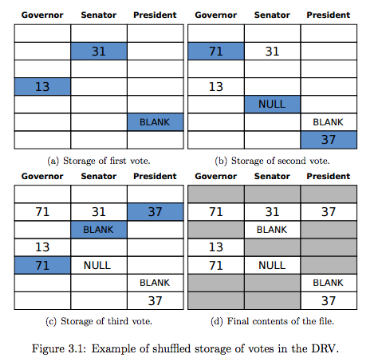
\includegraphics{Imagenes/privacidad1}
\caption{Ejemplo de votos en DRV}
\end{figure}

Se encontraron tres vulnerabilidades:
\begin{itemize}
	\item Una inadecuada elección del generador de números pseudo-aleatorios. Se utilizan las funciones rand y srand de C que tienen un periodo muy corto y aceptan solo semillas de 32 bits.
	\item Mala elección de la semilla. La semilla es el horario de apertura de la mesa de votación, que es durante las 7AM y 8AM, dando tan solo 3600 posibilidades.
	\item Semilla publica. No solo que el proceso de elección de la semilla es deterministica, sino que también se la publica en la documentación oficial de la mesa.
\end{itemize}

Dadas estas vulnerabilidades, se puede realizar los dos siguientes tipos de ataque:
\begin{itemize}
	\item Ataque directo: Se obtiene la semilla de la documentación oficial de la mesa, y se simula el movimiento de shuffle con N votos y se detecta en qué posición de la DRV fue almacenado cada voto. Esto permite obtener los votos en orden tan solo mirando la documentación oficial. Se pierde el anonimato de la votación si se conoce el orden en que los votantes emitieron sus votos.
	\item Ataque indirecto: Dado los votos fuera de orden, es posible realizar una búsqueda exhaustiva en los posibles valores de semillas, que son 3600, comparando los espacios vacíos.  Con la semilla correcta, se puede realizar el primer ataque
\end{itemize}

\subsection{Argentina}

\subsection{India}

\subsection{Israel}